\subsection{Störung}
Die Abmessungen des Acrylblocks werden mittels einer Schieblehre bestimmt. Die gemessenen Werte sind in der Tabelle \ref{tab:störung} dargestellt.
Die Gesammthöhe des Blockes beträgt $L = \SI{80,4}{mm}$. $\Delta L$ berechnet sich durch
\begin{align}
 \Delta L = L-L_{\text{a}}-L_{\text{c}}
 \label{eqn:L}
\end{align}
$L_a$ beschreibt den Abstand der Störung zur oberen Fläche das Blockes. $L_c$ ist dementsprechend die Entfernung nach unten.
\begin{table}[h!]
  \centering
  \caption{Abmessung es Acrylblocks}
  \label{tab:störung}
  \begin{tabular}{c c c c}
    \toprule
      Störung & $L_{\text{a}}$/ mm &$L_{\text{c}}$/mm &$\Delta L$/mm\\
    \midrule
1  & 19,5 & 59,5 & 1,4\\
2  & 17,8 & 61,2 & 1,4\\
3  & 61,4 & 13,2 & 5,8\\
4  & 54,0 & 21,6 & 4,8\\
5  & 47,6 & 30,2 & 2,6\\
6  & 39,0 & 38,5 & 2,9\\
7  & 31,1 & 46,6 & 2,7\\
8  & 23,1 & 54,7 & 2,6\\
9  & 15,0 & 62,0 & 3,4\\
10 &  7,0 & 70,4 & 3,0\\
    \bottomrule
  \end{tabular}
\end{table}

%\begin{figure}[h!]
%  \centering
%  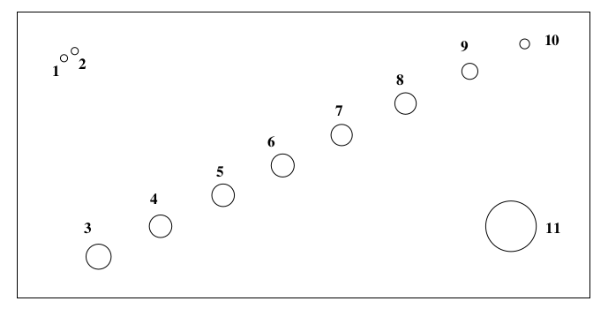
\includegraphics[width=0.9\textwidth]{Störungen.png}
%  \caption{Abbildung des Acrylblock \cite{1}}
%  \label{fig:acry}
%\end{figure}
\FloatBarrier

\subsection{A-Scan}
Der Acrylblock wird mit dem A-Scan untersucht. Die gemessenen Werte sind in der Tabelle \ref{tab:ascan} zu sehen.
Mit der Gleichung \ref{eqn:L} lässt sich $\Delta L$ bestimmen.
\begin{table}[h!]
  \centering
  \caption{Größe der Störung}
  \label{tab:ascan}
  \begin{tabular}{c c c c}
    \toprule
      Störung & $L_{\text{a}}$/ mm &$L_{\text{c}}$/mm &$\Delta L$/mm\\
    \midrule
3  &   63 & 14,2 &3,2\\
4  &   55 & 22,7 &2,7\\
5  &   47 & 31,4 &2,0\\
6  &   40 & 39,9 &0,5\\
7  &   32 & 47,9 &0,5\\
8  &   24 & 56,1 &0,3\\
9  &   16 & 64,0 &0,4\\
10 &    8 & -    &-\\
    \bottomrule
  \end{tabular}
\end{table}

Für die Bestimmung des Auflösungsvermögen werden die Störungen 1 und 2 genauer untersucht.
Dazu wird aus a-Richtung(Oben) und b-Richtung(Links) gescant.
Es ergeben sich die Werte:
\begin{align*}
  \text{Störung}_1: a=\SI{20,6}{mm}  && ,  b=\SI{15,4}{mm}\\
  \text{Störung}_2: a=\SI{18,9}{mm}  && ,  b=\SI{17,2}{mm}
\end{align*}
Mit einer höheren Frequenz kann das Auflösungsvermögen gesteigert werden.
Dies hat zur Folge, dass die Eindringtiefe kleiner wird.
Damit eine Struktur erfasst werden kann muss die Wellenlänge kleiner sein als die Störung.
Die Geschwindigkeit der Schallwellen im Acrylblock beträgt $v=\SI{2730}{\frac{m}{s}}$ und die Frequenz $f=\SI{2}{MHz}$.
Mit der Formel:
\begin{align*}
  \lambda = \frac{v}{f}
\end{align*}
ergibt sich ein Wert von
\begin{align}
  \lambda=\SI{1,365e-3}{m}=\SI{1,365}{mm}.
  \label{eqn:a}
\end{align}
Das heißt, wenn die Störung im Acrylblock kleiner ist als $\SI{1,365}{mm}$ kann sie von einer $\SI{2}{MHz}$ Frequenz
nicht mehr wahrgenommen werden.\\
In der Abbildung \ref{fig:ascan} ist eine Messung dargestellt.
Es wird die reflektierte Intensität in Volt in Bezug auf die Reflexionszeit gemessen.
Die Reflexionszeit wird zur Eindringtiefe umgerechnet.
Der erste Ausschlag ist die Reflektion der Wellen an den Grenzflächen: Schallkopf zu Wasser und Wasser zu Acryl.
Der zweie Peak wird durch die Störung verursacht.
Der dritte durch die Reflektion an der Tischplatte unter dem Acrylblock.
\begin{figure}[h!]
  \centering
  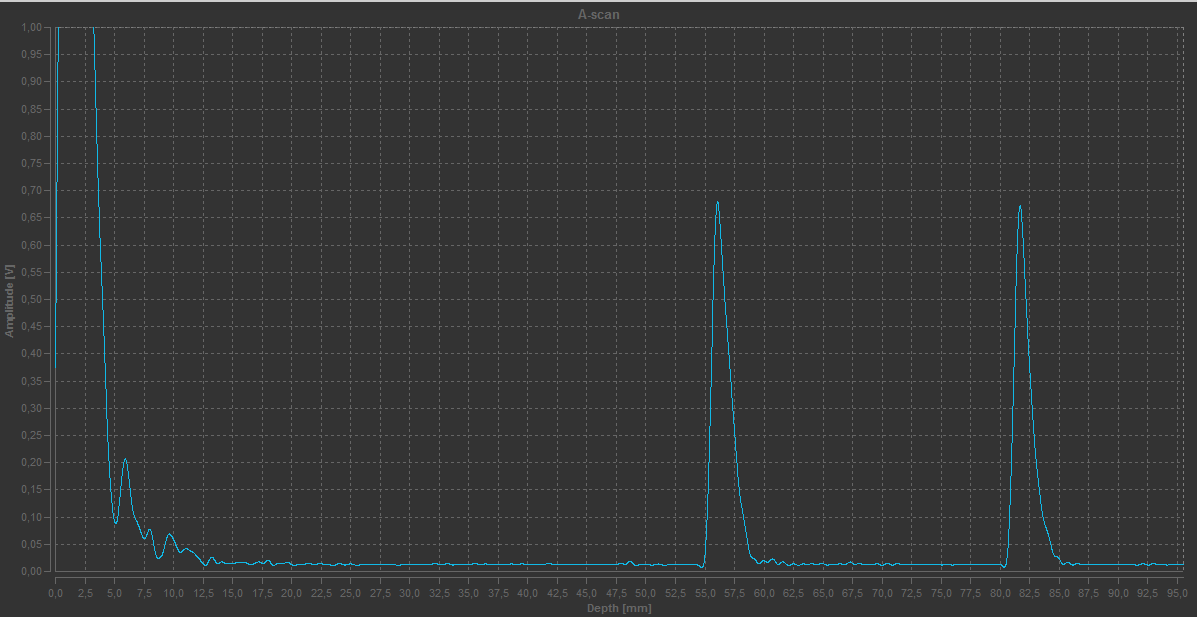
\includegraphics[width=0.9\textwidth]{ascan.png}
  \caption{A-Scan \cite{1}}
  \label{fig:ascan}
\end{figure}
\FloatBarrier

\subsection{B-Scan}
Nun werden die Störstellen mit dem B-Scan untersucht.
Die Messergebnisse sind in der Tabelle \ref{tab:bscan} aufgefürt.
Von jeder Seite werden pro Störung zwei Messwerte, Anfangs- und End- Punkt, aufgenommem.
Daraus läst sich jeweils die Größe der Störung bestimmen.
Desweiteren kann die Größe der Störung durch die Formel \ref{eqn:L} bestimmt werden.
\begin{table}[h!]
  \centering
  \caption{Größe der Störung}
  \label{tab:bscan}
  \begin{tabular}{c c c c c c c c}
    \toprule
      Störung & $L_{\text{a1}}$/ mm & $L_{\text{a2}}$/ mm & $\Delta L_{\text{a}}$/ mm & $L_{\text{c1}}$/mm & $L_{\text{c2}}$/ mm & $\Delta L_{\text{c}}$/ mm & $\Delta L_{\text{a1,c1}}$/mm\\
    \midrule
3  & 61,7 & 66,3 & 4,6  & 13,3 & 17,2 & 3,9 & 5,4\\
4  & 54,2 & 58,4 & 4,2  & 22,0 & 26,0 & 4,0 & 4,2\\
5  & 46,4 & 49,6 & 3,2  & 30,5 & 34,6 & 4,1 & 3,5\\
6  & 39,2 & 43,2 & 4,0  & 39,0 & 43,3 & 4,3 & 2,2\\
7  & 31,2 & 34,6 & 3,4  & 46,9 & 50,8 & 3,9 & 2,3\\
8  & 23,3 & 26,6 & 3,3  & 55,2 & 59,1 & 3,9 & 1,9\\
9  & 15,2 & 18,2 & 3,0  & 63,1 & 66,6 & 3,5 & 2,1\\
10 &  7,3 & 10,4 & 3,1 & -    & -    & -   & -  \\
    \bottomrule
  \end{tabular}
\end{table}

\begin{figure}[h!]
  \centering
  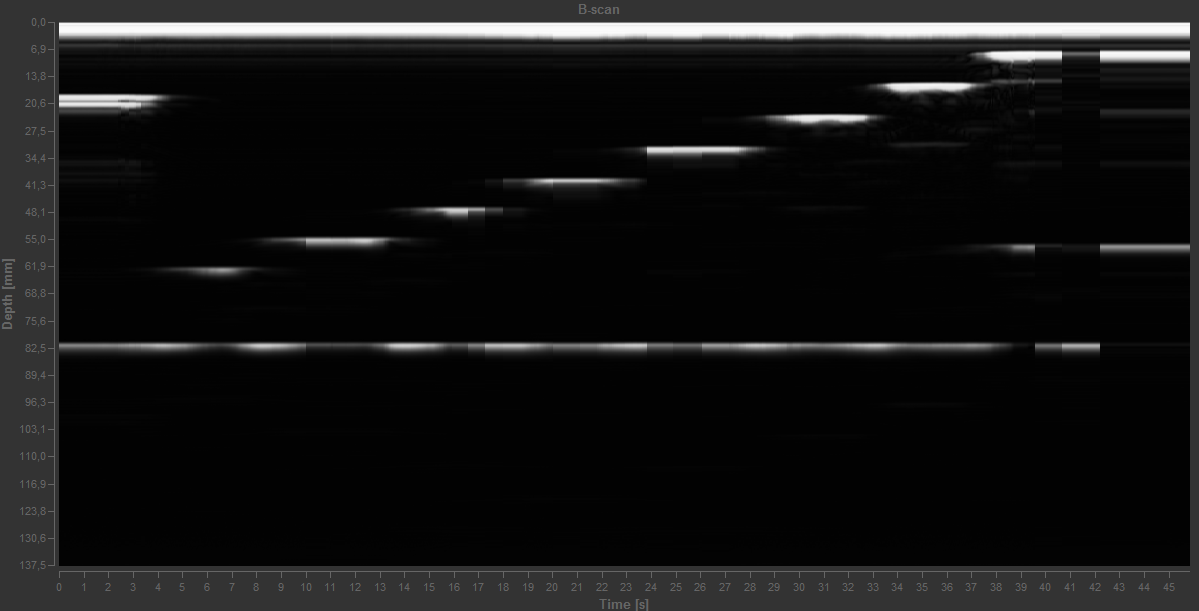
\includegraphics[width=0.9\textwidth]{bscan.png}
  \caption{B-Scan \cite{1}}
  \label{fig:bscan}
\end{figure}
\FloatBarrier

\subsection{Herzmodoell}
Am Herzmodellwird das soll das Herzvolumen untersucht werden.
Es wird die Entfernung der Membran zum Sonde gemessen.
Diese wird in Endsystolisch (Anspannung) und Enddiastolisch (Entspannung) eingeteilt.
Das verdrängte Volumen wird als Zylinder
\begin{align*}
  V=\pi r^2 \cdot h
\end{align*}
genähert. h ist dabei die Höhe als endsystolische Höhe abzüglich der enddiastolischen Höhe.
\\Folgende Werte werden gemessene:
\begin{align*}
  \text{Endsystolisch}&=\SI{30,7}{mm}\\
  \text{Enddiastolisch}&=\SI{27,1}{mm}\\
  \text{Durchmesser}&=\SI{45,8}{mm}\\
  \nu&=\SI{2}{\frac{1}{s}}
\end{align*}
Mit den Messwerten kann das Herzvolumen wie folgt berechnet werden.
\begin{align*}
\text{Volumenänderung}&=\pi\cdot (\SI{22,9}{mm})^2\cdot(\SI{30,7}{mm}-\SI{27,1}{mm})\\
  \text{Volumenänderung}&=\SI{5930,09}{mm}^3\\
  \text{Herzvolumen} &= \text{Volumenänderung}\cdot \nu\\
  \text{Herzvolumen} &= \SI{11861,87}{\frac{mm^3}{s}}=\SI{1,18e-5}{\frac{m^3}{s}}
\end{align*}
\begin{figure}[h!]
  \centering
  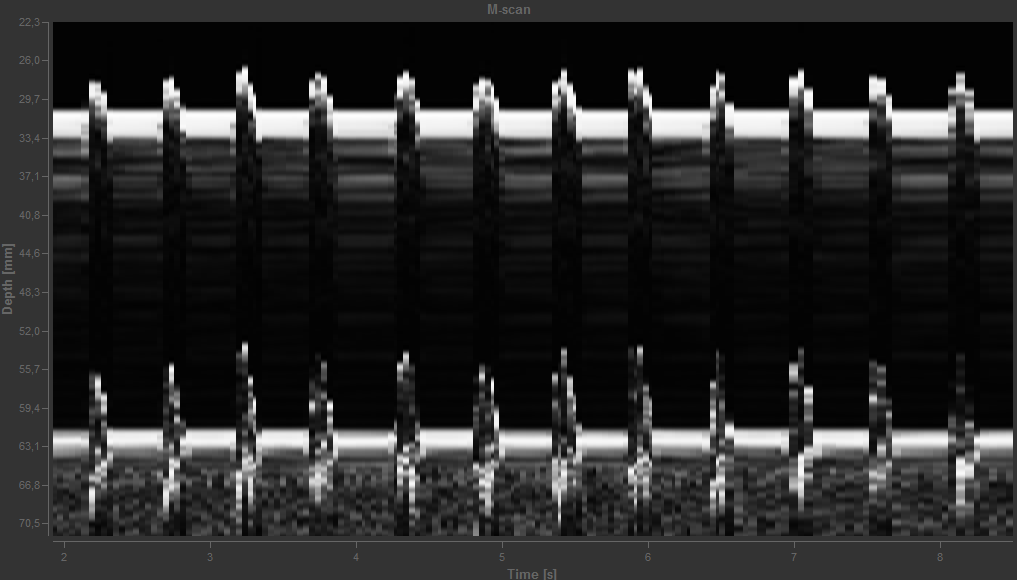
\includegraphics[width=0.9\textwidth]{herz.png}
  \caption{Messung am Herzmodell \cite{1}}
  \label{fig:herz}
\end{figure}
